% INTRO %
This sections is concerned with the objectives, methodology, and results from the \textit{Feasibility Test (FT)}.

% GOALS %
The \textit{FT} covers two objectives: \textbf{(1)} validate the environment described in the previous section, allowing the \textit{implementation stage} to be carried out over it, and \textbf{(2)} render the possibility to develop a \textit{XDP} program and test its execution.

% METHODOLOGY %
The \hyperref[sec:Introduction]{Introduction} regarded the implementation of \textit{XDP} through three different modes: \textbf{(1)} Generic \textit{XDP}, \textbf{(2)} Native \textit{XDP}, and \textbf{(3)} Offloaded \textit{XDP}.
The \textit{FT} is focused on Generic \textit{XDP}, since it allows the accomplishment of the aforementioned objectives without the need for supporting hardware.
The developed program models the drop of all packets except for IPv6.

\noindent \textbf{Methodology (step by step):}
\begin{itemize}
    \item Develop the program;
    \item Build the object;
    \item Load the object;
    \item Experiment the environment
\end{itemize}

% CODE %
\noindent \textbf{\textit{XDP} program:}
\lstinputlisting[language=C, caption=\textit{C} program to drop all packets but IPv6.]{src/xdp_pass_ipv6.c}

\textit{SEC} enables the placement of compiled object fragments into different \textit{Executable and Linkable Format (ELF)} sections.
The function \textit{xdp\_pass\_ipv6} accepts a parameter of type \textit{struct xdp\_md*}.
This struct allows the initialization of pointers referencing crucial header delimiters, being used to assert the access of legal fields within the header.
If the protocol used is IPv6, the packet is passed, through the return of \textit{XDP\_PASS}.
Otherwise, the packets are dropped while returning \textit{XDP\_DROP}.
Finally, the last line regards to the license associated with the program, that being \textit{General Public License (GPL)}\cite{XDPRedHat}.

% LOAD %
\noindent \textbf{Loading:}

\begin{lstlisting}[language=Bash]
$ sudo ip link set interface xdpgeneric obj xdp_pass_ipv6.o sec xdp_pass_ipv6
\end{lstlisting}

The \textit{ip} command is expressive enough to load the object in question, however, \textit{xdp\_loader} from \textit{xdp-tools}, offers greater capabilities and will be use in advanced scenarios.

% EXPERIMENT %
\noindent \textbf{Experimentation:}

Commands such as \textit{xdp-loader status}, \textit{bpftool prog show}, \textit{ip link show}, \textit{ping}, among other network debugging tools where used to experiment on \textit{XDP}.

\begin{figure}[h]
    \centering
    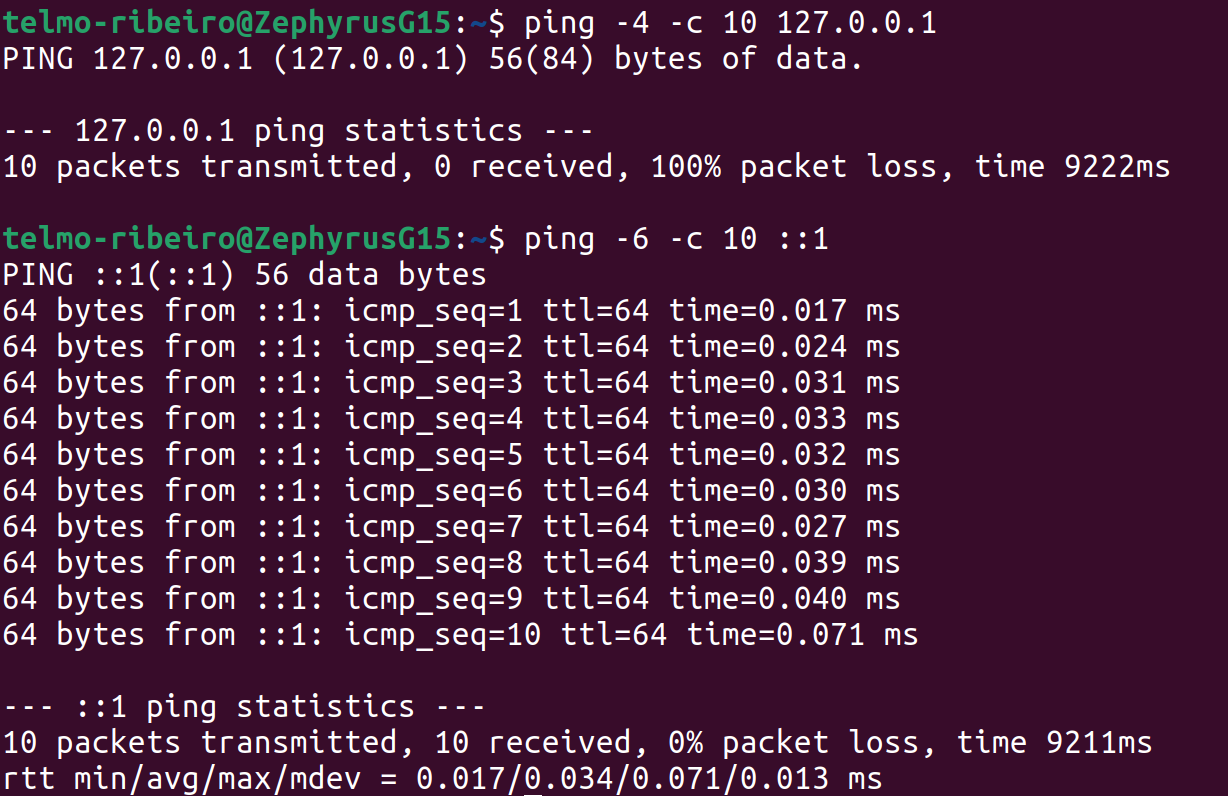
\includegraphics[width=250pt]{src/figures/ping-test.png}
    \caption{ping output for the loopback interface}
    \label{fig:ping-test}
\end{figure}

Figure \ref{fig:ping-test} displays ping command's output over ICMPv4 and ICMPv6 regarding the loopback interface loaded with the aforementioned object.
Although this output alone does not constitute a proof of correctness on \textit{xdp\_pass\_ipv6}, and thus came the need for multiple tests and debugging tools, it was a reliable indication on the program well behaviour.   

% RESULTS %
The tests performed on the interface, corroborated the \textit{XDP} program correctness, therefore, deriving the objectives achievement for the \textit{FT}.